\documentclass[11pt,openany]{book}
% #1-Asignatura
% #2-Curso
% #3-Nombre
% #4-Link
% #5-Foto

\newcommand{\portada}[5]{
    \begin{titlepage}
        \begin{center}
            \vspace*{0.5cm}
            
            % Titulo con #1 lo mas grande posible
            {\Huge \textbf{#1}}

            
            \vspace{0.5cm}
            \LARGE
            Curso #2 
            
            \vspace{1cm}
            
            \Huge{\textbf{Grupo Viterbi}}

            \vspace{1cm}
            
\includegraphics[width=0.6\textwidth]{assets/Img/UGR-Logo.png}
            
            \vspace{0.5cm}

            \huge
            PRÁCTICA 5- PROGRAMACIÓN DINÁMICA
            
            \Large
            \vspace{1cm}
            \textbf{Integrantes:}  \\ 
             % Array con los nombres de los integrantes y el correo
             \begin{center}
                \begin{tabular}{c c }
                    \textbf{Miguel Ángel De la Vega Rodríguez} & miguevrod@correo.ugr.es \\
                    \textbf{Alberto De la Vera Sánchez} & joaquinrojo724@correo.ugr.es \\
                    \textbf{Joaquín Avilés De la Fuente} & adelaveras01@correo.ugr.es \\
                    \textbf{Manuel Gomez Rubio} & e.manuelgmez@go.ugr.es \\
                    \textbf{Pablo Linari Perez} & e.pablolinari@go.ugr.es
                \end{tabular}
             \end{center}
            \vspace{0.8cm}
            
            
            \large
             \vspace{1cm}
            Facultad de Ciencias UGR\\
            Escuela Técnica Ingeniería Informática UGR\\
            Granada\\
            #2 
            
        \end{center}
    \end{titlepage}
}



\usepackage{assets/formulas}
\usepackage[mathscr]{euscript}
\usepackage{bm}
\usepackage{float}
\hbadness=10000 % Suppress Underfull \hbox warnings

%========================================|Indice|===============================================%

\begin{document}
\portada{Algorítmica}{2023-2024}{Miguel Ángel De la Vega Rodríguez}{https://github.com/Miguevrgo/}{github.png}
\tableofcontents % Índice
\newpage %Salto de pagina tras el Indice


%======================================|Documento|==============================================%
\chapter{Autores}
\begin{itemize}
      \item \textbf{Miguel Ángel De la Vega Rodríguez:} 20\%
            \begin{itemize}
                  \item Algoritmos Greedy del Viajante
                  \item Redacción memoria sección Viajante
            \end{itemize}
      \item \textbf{Joaquín Avilés De la Fuente:} 20\%
            \begin{itemize}
                  \item Programacion Dijkstra
                  \item Programación creación de grafos (casos de prueba)
                  \item Redacción memoria sección Dijkstra
            \end{itemize}
      \item \textbf{Alberto De la Vera Sánchez: } 20\%
            \begin{itemize}
                  \item Redacción \LaTeX
                  \item Estudio de umbrales teóricos y empíricos de DyV
                  \item Graficas y ajustes
            \end{itemize}
      \item \textbf{Manuel Gomez Rubio} 20\%
            \begin{itemize}
                  \item Programacion SumaMax (Kadane)
                  \item Programacion Losetas
            \end{itemize}
      \item \textbf{Pablo Linari Pérez:} 20\%
            \begin{itemize}
                  \item Programacion SumaMax (Kadane)
                  \item Programacion Losetas
            \end{itemize}
\end{itemize}

\chapter{Equipo de trabajo}

\begin{itemize}
      \item \textbf{Miguel Ángel De la Vega Rodríguez:} (Ordenador donde se ha realizado el computo)
            \begin{itemize}
                  \item AMD Ryzen 7 2700X 8-Core
                  \item 16 GB RAM DDR4 3200 MHz
                  \item NVIDIA GeForce GTX 1660 Ti
                  \item 1 TB SSD NvMe
                  \item Debian 12 Bookworm
                  \item Compilador GCC 12.2.0
            \end{itemize}
\end{itemize}

\chapter{Asignación de aulas}
En esta sección se estudia lo referente al algoritmo usado para resolver el segundo 
problema el cual nos pide lo siguiente :

Se quieren ralizar N exámenes en un día en la ETSIIT , el centro cuenta con m aulas donde m es mayor
que N . Sin embargo cada vez que se utiliza un aula el centro debe contratar un vigilante por tanto 
se debe diseñar un algoritmo que clacule en base al horario de los exámenes el menor costo posible 
para la escuela , es decir hay que encontrar la manera de distribuir los exámenes para usar el menor número
de aulas posibles .

\section{Estructura de los datos}
Una vez planteado el problema porcedemos a describir las herramientas que hemos usado para resolverlo 
Para representar los horarios de los exámenes hemos usado la siguiente estructura :

\begin{lstlisting}
      struct tiempo{
            int hora;
            int min;
            tiempo(int h , int m){
                hora = h;
                min = m ;
            }
      };
      struct examen{
            tiempo inicio; // Hora de inicio
            tiempo final; // Hora de finalizacion
            examen(tiempo t , tiempo t1) : inicio(t), final(t1){}
      };
        
      struct compare{
            bool operator()(const examen&a,const examen&b){
                if(a.inicio.hora==b.inicio.hora){
                    return a.inicio.min < b.inicio.min;
                }
                return a.inicio.hora < b.inicio.hora;
            }
      };
        
\end{lstlisting}

El struct compare se utiliza para ordenar el vector de entrada de exámenes de manera que se ordenen
de menor a mayor en función de la hora de inicio de los exámenes , de esta manera se facilita la
ejecución del algoritmo que se encarga de asignar los exámenes a las aulas de la manera más eficiente
posible.

\section{Algoritmo}

A continuación vemos el algoritmo usado para la distribución de las aulas.

\begin{lstlisting}[language=C++]
      bool sesolapan(examen e1,examen e2){
            if(e1.final.hora == e2.inicio.hora){
                return e1.final.min >e2.inicio.min;
            }
            return e1.final.hora > e2.inicio.hora;
        }
        
        int minAulas(const vector<examen> & v){
        
            // Conjunto de candidatos v
        
            int naulas = 1;
            vector<queue<examen>> horario;
            //Conjunto de seleccionados horario (vector de colas , cada cola es un aula)
            
            horario.emplace_back(queue<examen>());
            horario[0].push(v[0]);
            int i;
            //
            for(int nex = 1;nex < v.size();nex++){
                i=0;
                //Funcion de seleccion
                while(i<horario.size() && (sesolapan(horario[i].back(),v[nex]))){i++;}
                //Funcion de factibilidad
                if(i==horario.size()){
                    horario.emplace_back(queue<examen>());
                    horario[i].push(v[nex]);
                    naulas++;
                }
                else{
                    horario[i].push(v[nex]);
                }
            }
            return naulas; //Funcion objetivo 
      }
\end{lstlisting}

Uno de los factores importantes que hay que destacar de este algoritmo es que el vector \textbf{v} se supone 
ordenado de mayor a menor , es decir que en el vector los exámenes aparecen en orden creciente de 
horario de inicio de esta manera la asignación de aulas es más rápida y eficiente.

El algoritmo comienza añadiendo el primer examen al primer aula , cada aula se representa con una posición del vector 
y el horarario del aula se representa con una cola ya que solo nos interesa el último examen hecho en el aula.

Posteriormente se entra al bucle for el cual recorre todo el vector de candidatos ya que todos los exámenes deben
ser realizados . 

Dentro del bucle for se entra a un while el cual comprueba mediante la función \textbf{sesolapan(examen e1 ,examen e2)}
si el examen que está buscando un aula se solapa con el que se está realizando en el aula , si no se solapan se añade a 
ese aula , si se solapan se busca otra aula en la que no se solapen y se añade a esa aula. En el caso de que se hallan agotado
las aulas actuales se crea una nueva aula y se añade el examen a esa aula.

\section{Justificación Greedy}

En este apartado vamos a analizar el algoritmo identificando los componentes que lo hacen un algoritmo greedy 
y demostrando que siempre llega a la solución óptima. 


\chapter{Camino mínimo} % Manuel y Joaquin
En esta sección se analiza todo lo relacionado con el tercer problema propuesto, el problema del camino mínimo entre dos ciudades. 
Comentaremos el algoritmo usado, es decir, el \textbf{algoritmo de Dijkstra}, y su implementación en C++, así como la justificación de su uso mediante
la demostración de que dicho algoritmo Greedy calcula la solución óptima.  \\
Destacar también que mostraremos la gestión que hemos hecho para la creación de los posibles casos (\textbf{grafos}), así como la 
ejecución de los mismos y la obtención de los resultados.

\section{Algoritmo de Dijkstra (DEMOSTRACION)}
A continuación, veremos las distintas partes usadas para la demostración como bien pueden ser la función de selección, así como
la forma en que se seleccionan los nodos, y finalmente la demostración mediante inducción. \\
Definiremos pues cada parte del algoritmo: \\
\begin{itemize}
      \item Candidatos a seleccionar:\\
            En este problema los candidatos a seleccionar son los diferentes vértices del grafo que no hayan sido \\
            seleccionados previamente.
      \item Candidatos seleccionados:
            Llamaremos $\mathscr{S}$ al conjunto de los vértices seleccionados. \\
            En nuestro problema siempre partiremos de un vértice, por lo que, como mínimo siempre habrá un vértice en $\mathscr{S}$ que será el origen 
            desde donde partiremos a considerar los nuevos vértices.

            Una vez definido $\mathscr{S}$ hay que definir también $\mathscr{V}\setminus\mathscr{S}$ que será el conjunto de vértices candidatos a ser seleccionados,
            siendo por tanto, $\mathscr{V}$ el total de vértices del grafo.

      \item Función Solución:\\
            La solución se obtendrá cuando el nodo origen y el destino estén en $\mathscr{S}$, siendo el ndo destino el último seleccionado, teniendo así el camino mínimo $\mathscr{M}(o,v)$

      \item Función de Selección:\\ 
            La función de selección en este algoritmo es siempre tomar el camino de menor distancia posible entre los nodos que estén conectados con el origen, actualizando los nuevos posibles candidatos 
            tras una elección

      \item Función de factibilidad:\\
            Un vértice es seleccionable en el caso enel que su distancia respecto al origen no sea infinito, esto quiere decir que debe haber vérices dentro de los seleccionados que nos permitan, mediante
            caminos directos, alcanzar el vértice sobre el que nos preguntamos si es factible

      \item Funcion objetivo: \\
            El problema tendrá siempre tamaño $\mathscr{V}$, es decir, el número de vértice del grafo. (Se puede considerar el tamaño real como $\mathscr{V}-1$ ya que el nodo de origen siempre es el primero en seleccionarse sin
            tener en cuenta ningún criterio)
\end{itemize}
Una vez definidas las funciones, conjuntos de candidatos... pasaremos a realizar la demostración del algortimo greedy.

\begin{itemize}
      \item Demostración Greedy: \\
            Para la demostración, usaremos inducción y reducción al absurdo.
      \item El caso base será cuando \#$\mathscr{S}=1$ o bien es igual a 2.\\
            En ambos casos el algorimo nos dará una solución trivial, ya que, en el caso \#$\mathscr{S}=1$ la distancia mínima entre un vértice consigo mismo es 0.
            En el caso de que \#$\mathscr{S}=2$, tenemos que la distancia mínima entre los dos nodos será la que los conecte con menor distancia, puesto que el grafo es conexo y no pueden no estar conectados.
      \item Paso de inducción:
            Sea $v$ el nuevo vértice que ha sido seleccionado por el algoritmo, y por tanto $v\in \mathscr{S}$.\\
            Ahora usaremos reducción al absurdo y tomaremos que la distancia $d(v)$ (que representa algún camino de $o$ a $v$, con $o$ como el nodo de origen) no es la longitud mínima.\\
            Tomaremos entonces, $\mathscr{L}$ como la distancia mínima de $o$ a $v$. Y tenemos en cuenta que en $\mathscr{L}$ hay un camino que parte de un nodo x, ($c(x,y)$ camino de x a y), siendo x el último nodo en $\mathscr{S}$\\
            Con todo esto tenemos:
            \begin{equation*}
                  \mathbf{d(v)}\bm{>}\mathscr{M}(o,v)=\mathscr{M}(o,x)+c(x,y)+\mathscr{M}(y,v) > \mathscr{M}(o,x)+c(x,y)= d(x)+c(x,y)=\mathbf{d(y)}
            \end{equation*}
            Donde hemos usado que $\mathscr{L}$ es el camino mínimo y está formado por la primera igualdad.\\
            En la primera desigualdad, usamos la hipótesis de inducción, puesto que suponíamos que $d(v)>\mathscr{L}$.
            Por último, nos falta explicar la contradicción que hemos obtenido, que está marcada en negrita.
            Esta contradicción nos indica que al ser la distancia de y menor que la de v, nuestro algoritmo debería haber elegido al vétice $y$ en vez de a $v$\\
            Luego, hemos probado la optimalidad de nuestro algoritmo.

\end{itemize}

\section{Estructura de datos y grafos}
Para la implementación del algoritmo de Dijkstra, hemos usado una estructura de datos que nos permita representar un grafo, en este caso,
hemos usado una matriz de adyacencia. Por tanto, a continación se explicara de forma detallada la creación de dichos grafos así como la forma de 
representarlos en archivos de texto, ya que al ser la primera vez que se trabaja con grafos es útil tener
claro como se ha hecho. \\ \\
Para la creación de los grafos se ha hecho uso de un programa en C++ que nos permite generar grafos aleatorios, a partir
de un vector que tenga los distintos puntos. Destacar en primer lugar, que para la creación de los puntos de forma aletoria hemos usado 
de este trozo de código:
\begin{lstlisting}[language=C++]
// Inicializar el generador de numeros aleatorios
srand(time(NULL));

// Generar puntos aleatorios y escribirlos en el archivo
for (int i = 0; i < numPuntos; i++) {
      int coordX = rand() % (rangoMax + 1); // Generar coordenada x
      int coordY = rand() % (rangoMax + 1); // Generar coordenada y
      file << coordX << " " << coordY << endl; // Escribir coordenadas al archivo
}
\end{lstlisting}
donde file es el archivo donde se escriben los puntos, numPuntos es el número de puntos que se quieren generar y rangoMax es el rango
máximo de las coordenadas. \\
Tenemos ahora archivos con distintos puntos aleatorios, y para la creación de los grafos, hemos usado el siguiente código:
\begin{lstlisting}[language=C++]
// Debe estar la matriz inicializada a 0
void creacionGrafos(const vector<Point>&vec, vector<vector<double>> &matriz){
      int size=vec.size();

      srand(time(NULL));

      for (int i=0; i<size; i++){
            // Num nodos que conectaremos con el nodo i
            int conexiones=rand()%(size-1)+1;
            for(int j=0; j<conexiones; j++){
            // Nodo a conectar con el nodo i
            int nodo_conectar;
            do{
                  nodo_conectar=rand()%size;
            } while(nodo_conectar==i);
            // Aniadimos su distancia a la matriz
            matriz[i][nodo_conectar]=vec[i].distanceTo(vec[nodo_conectar]);
            }
      }
      
      int p_inicio=rand()%size;

      for(int i=0; i<size; i++){
            matriz[p_inicio][i]=vec[p_inicio].distanceTo(vec[i]);
            matriz[i][i]=0;
      }

}
\end{lstlisting}
donde la matriz pasada por referencia será la llamada \textbf{matriz de adyacencia} que representa el grafo, y \textbf{vec} es el vector de puntos
leido del archivo. \\ \\
Las matrices de adyacencia que hemos obtenido, las hemos guardado en archivos de texto, para poder leerlas posteriormente y ejecutar
el algoritmo de Dijkstra sobre ellas, por lo que para ello hemos creado funciones que permitan leer y guardar dichas matrices, pues hay que recordar que 
los puntos que no tengan conexión directa, tendrán un valor de infinito en la matriz. Tenemos así estas dos funciones, una para 
escribir la matriz en un archivo de texto y otra para leerla:
\begin{lstlisting}
// Funcion para mostrar una matriz en un archivo
void mostrarMatriz(std::ofstream &salida, const std::vector<std::vector<double>>& matriz) {
      // Configurar la salida para mostrar numeros con tres decimales
      salida << std::fixed << std::setprecision(3);

      // Iterar sobre cada fila de la matriz
      for (const auto& fila : matriz) {
            // Iterar sobre cada elemento de la fila y mostrarlo
            for (double elemento : fila) {
            if(elemento==numeric_limits<double>::max())
                  salida << std::setw(5) << "INF" << "\t";
            else
                  // Asegurar que todos los numeros se alineen correctamente usando setw
                  salida << std::setw(5) << elemento << "\t"; // Separador de columnas
            }
            salida << std::endl; // Nueva linea para la siguiente fila
      }
}

// Funcion para leer la matriz desde un archivo
void lecturaMatriz(ifstream &leer, vector<vector<double>>& matrix) {
      string line;
      while (getline(leer, line)) {
            vector<double> row;
            stringstream ss(line);
            string val_str;
            while (ss >> val_str) {
            if (val_str == "INF") {
                  row.push_back(numeric_limits<double>::max());
            } else {
                  row.push_back(stod(val_str));
            }
            }
            matrix.push_back(row);
      }
}
\end{lstlisting}
donde \textbf{numeric\_limits<double>::max()} es el valor que hemos usado para representar la ausencia de conexión entre dos nodos, que
en la matriz escrita y leida se mostrará como \textbf{INF} de infinito.\\ \\
Finalmente, para la ejecución del algoritmo de Dijkstra, hemos usado el siguiente código:
\begin{lstlisting}
// Funcion auxiliar para encontrar el vertice con la distancia minima
int minDistance(const vector<double>& dist, const vector<bool>& visited) {
      double min = INF;
      int min_index = -1; // Inicializado a -1 para detectar errores si no se encuentra ninguno

      for (int v = 0; v < dist.size(); v++) {
            if (!visited[v] && dist[v] <= min) {
                  min = dist[v];
                  min_index = v;
            }
      }
      return min_index;
}
// Funcion para implementar el algoritmo de Dijkstra desde inicio hasta un nodo destino w
void dijkstra(const vector<vector<double>>& graph, int inicio, int final) {
      int V = graph.size();
      vector<double> dist(V, INF); // Distancias minimas
      vector<bool> visited(V, false); // Nodos visitados
      vector<int> parent(V, -1); // Para rastrear el camino

      // Inicializar la distancia del nodo inicial a si mismo como 0
      dist[inicio] = 0;
      
      for (int count = 0; count < V - 1; count++) {
            int u = minDistance(dist, visited);
            visited[u] = true;
      
            // Si el nodo seleccionado es el nodo destino, terminar el algoritmo
            if (u == final)
            break;
      
            for (int v = 0; v < V; v++) {
            if (!visited[v] && graph[u][v] != 0 && dist[u] != INF && dist[u] + graph[u][v] < dist[v]) {
                  dist[v] = dist[u] + graph[u][v];
                  parent[v] = u; // Registrar el nodo padre para rastrear el camino
            }
            }
      }
      
      // Imprimir la distancia minima
      cout << "Distancia minima desde el nodo " << inicio << " al nodo " << final << ": " << dist[final] << endl;

      // Imprimir el camino recorrido
      printPath(parent, inicio, final);
}
       
\end{lstlisting}
donde hemos definido \textbf{const double INF = numeric\_limits<double>::max()} para representar la ausencia de conexión entre dos nodos.
La función \textbf{minDistance} nos permite encontrar el nodo con la distancia mínima, y la función \textbf{dijkstra} nos permite ejecutar
el algoritmo de Dijkstra desde un nodo inicial hasta un nodo final, mostrando la distancia mínima y el camino recorrido, haciendo uso
de la función \textbf{printPath} que se muestra a continuación:
MOSTRARLAAAAAAAAAAAAAAAAAAAAAAAAAAAAAAAAAAAAAAAAAAA
% //TODO: Añadir la función printPath


% Viajante es el apartado 6, incluir capitulos antes
\chapter{Viajante} % Migue
En esta sección se analiza todo aquello referente al cuarto problema propuesto,
el problema del viajante. Siguiendo las directrices indicadas, se han estudiado
y diseñado diferentes algoritmos "Greedy" que aproximan el problema, con el objetivo
final de comparar cual nos proporciona mejores resultados en cuanto a términos
de eficiencia y precisión. Para determinar esto último, también cabe destacar
detalles de menor importancia como la complejidad de los algoritmos, la estabilidad
frente a distintas entradas o la posibilidad de mejora de los mismos mediante la
elección de distintos puntos de partida o con mejoras posteriores como pueden ser 
aquellas que proporcionan algoritmos como $\lambda$-opt o genéticos.
\\ \\
De aqui en adelante, describiremos por secciones los algoritmos implementados y 
al final proporcionaremos una sección comparativa sobre la cual nos basaremos
para determinar conclusiones, en particular, elegiremos el algoritmo cuya
solución consideremos más conveniente. En lo que sigue se muestra únicamente
el resultado obtenido por el algoritmo sin mejoras posteriores, este tipo de mejoras
suponen una pequeña desvirtuación del objetivo de encontrar el mejor algoritmo y 
es por ello, que su uso se limita a la conclusión final.

\section{Algoritmo \textit{Nearest Neighbour}}
Tal y como el nombre indica, el primer algoritmo implementado no es nada más, ni 
nada menos que el primer algoritmo que probablemente se le puede ocurrir a cualquier
persona que se enfrente a este problema. La idea es sencilla e intuitiva, nos 
dan un conjunto de puntos y queremos encontrar el camino más corto que los recorra,
para ello, \textbf{elegimos} un punto inicial y a partir de ese punto, en un proceso 
iterativo, elegimos en cada paso el siguiente punto más cercano al actual, o lo que 
es lo mismo, el punto para el cual la distancia al punto actual es la menor (No confundir
con el punto para el cual la distancia total es la menor, ya que, aunque parecido, no es 
lo mismo). Este proceso se repite hasta que todos los puntos han sido visitados.
\\ \\
A continuación se proporciona la implementación propuesta del algoritmo en cuestión:
\begin{lstlisting}[language=C++]
vector<Point> nearestNeighborTSP(const vector<Point>& points) {
  vector<Point> path;
  vector<bool> visited(points.size(), false);
  path.reserve(points.size());
  path.emplace_back(points[0]);
  visited[0] = true;

  for (int i = 0; i < points.size() - 1; ++i) {
    double minDistance = numeric_limits<double>::max();
    int nearestNeighbor = -1;
    for (int j = 0; j < points.size(); ++j) {
      if (!visited[j]) {
        double distance = path[i].distanceTo(points[j]);
        if (distance < minDistance) {
          minDistance = distance;
          nearestNeighbor = j;
        }
      }
    }
    path.emplace_back(points[nearestNeighbor]);
    visited[nearestNeighbor] = true;
  }

  return path;
}
\end{lstlisting}
Como se puede apreciar, se ha hecho uso de un vector de puntos visitados (Programación 
dinámica) para evitar visitar un punto más de una vez, esto no supone una complejidad
notable, sin embargo, si que supone una gran mejora en términos de eficiencia.

\section{Algoritmo \textit{Ordenación}}
Como el nombre indica, este algoritmo consiste en ordenar los puntos de partida de
acuerdo a un criterio especifico (en nuestro caso los hemos ordenado por la coordenada
x de menor a mayor, teniendo en cuenta también para puntos cercanos en x, la coordenada y).
Una vez ordenados los puntos, simplemente recorremos el vector de puntos en el orden
en el que se encuentren, de esta forma, el camino total trata de reducir cruces y distancias
con la idea intuitiva de que si dos puntos están cerca en el plano, probablemente, la 
distancia que se recorra al pasar por ellos, sea mínima. Como veremos en el siguiente 
algoritmo y en la conclusión, esto en la práctica no es del todo cierto. Primero veamos 
la implementación del algoritmo:
\begin{lstlisting}[language=C++]
vector<Point> orderedTSP(const vector<Point>& points) {
      vector<Point> tour;
      tour.reserve(points.size());
      copy(points.begin(), points.end(), back_inserter(tour));
      sort(tour.begin(), tour.end());
        
      return tour;
}      
\end{lstlisting}
Como se puede apreciar, la implementación es muy sencilla, simplemente se copian los puntos
de partida a un vector auxiliar, se ordenan y se devuelve el vector ordenado, sin embargo
cuando vemos el resultado de la ejecución, nos damos cuenta de que aunque los puntos
esten muy cerca respecto a la coordenada x, los saltos que se dan en la coordenada y
pueden ser muy grandes, lo que hace que el camino total sea mucho mayor de lo esperado,
además para cerrar el camino, la distancia es la máxima posible en cuanto a x. Para mejorar
esto, podemos observar que si nuestro problema son los saltos en la coordenada y 
y la distancia de cierre, podemos intentar minimizarlos, de donde surge el siguiente
algoritmo.

\section{Algoritmo \textit{Circular}}
Para solucionar el problema anterior, se propone una alternativa que se basa en la misma
idea de ordenar por la coordenada x, sin embargo, en este caso la coordenada y solo se tiene 
en cuenta tras ordenar, lo que se hace es guardar el la coordenada y de los puntos máximo
y mínimo y se calcula el punto medio entre ambos, esto se hace para recorrer los puntos
de forma circular como el nombre indica, de modo que los puntos que se quedan en la parte 
de abajo del plano, se recorren en sentido horario y los puntos que se quedan en la parte
de arriba del plano, se recorren en sentido antihorario. De esta forma, se consigue minimizar
la cantidad de saltos en el eje y y la distancia de cierre, resulta sugerente pensar que este 
proceso de división en dos partes, se puede hacer de forma recursiva, sin embargo, en la 
práctica, esto supone una complejidad superior a la hora de implementar mas bucles, y no
supone una mejora significativa en términos de precisión, por lo que se ha optado por
dejarlo de esta forma. 
\\ \\
El problema que presenta esta implementación es que dependiendo de la forma que tenga
el conjunto de puntos que se le pase, se obtendrán resultados muy distintos, sin embargo
esto ocurre en todos los algoritmos, por lo que no se considera un problema en si mismo, 
ya que es inherente al problema. A continuación se muestra la implementación del algoritmo:
\begin{lstlisting}[language=C++]
vector<Point> CircTSP(const vector<Point>& points) {
    vector<Point> tour;
    vector<Point> circularTour;
    tour.reserve(points.size());
    circularTour.reserve(points.size());
    tour = points;
    sort(tour.begin(), tour.end());
    
    int min = numeric_limits<int>::max();
    int max = numeric_limits<int>::min();

    for (int i = 0; i < points.size(); ++i) {
        min = min(min, points[i].getY());
        max = max(max, points[i].getY());
    }
    
    double mid = (max + min )/2;

    for (int i = 0; i < points.size(); ++i) {
        if (tour[i].getY() <= mid) {
            circularTour.emplace_back(tour[i]);
        }
    }

    for (int i = points.size(); i >= 0; --i) {
        if (tour[i].getY() > mid) {
            circularTour.emplace_back(tour[i]);
        }
    }

    return circularTour;
}
\end{lstlisting}

Una vez mas, podemos apreciar que se puede aumentar la eficiencia del algoritmo
optimizando bucles y la ordenación de manera que el máximo y el mínimo se calculen
mientras se ordenan los puntos, sin embargo, esto no supone una mejora en cuanto
al orden de eficiencia y si supone una mayor complejidad del codigo, por lo tanto,
como el compilador se encarga de optimizar esos detalles que no afectan al orden
de eficiencia, se ha optado por dejarlo de esta forma para facilitar la lectura, 
en una implementación real, se recomendaría la optimización manual de estos detalles, ya que,
aunque bueno, el compilador no es perfecto y no siempre optimiza de la mejor forma.
\section{Conclusiones}
Una vez presentados los tres algoritmos, nos disponemos a obtener conclusiones acerca
de ellos así como a compararlos para determinar cual es el mejor, o cómo podríamos
mejorar la precisión de los mismos. Comenzamos mostrando visualmente los resultados
de ejecución de cada uno de ellos, con el objetivo de que el lector pueda apreciar 
de forma sencilla la idea que se ha querido transmitir con cada uno de los algoritmos.
\subsection{Graficas}
% Dos graficas en una fila y una debajo
\begin{figure}[H]
      \centering
      \begin{minipage}{.48\textwidth}
            \centering
            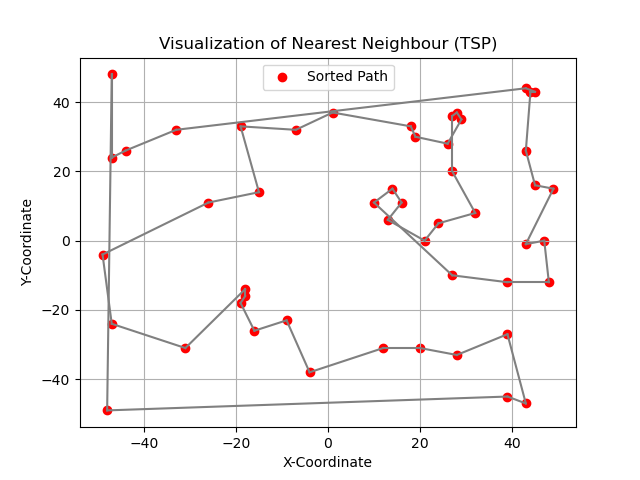
\includegraphics[width=1.1\linewidth]{assets/Img/NearestVisual.png}
            \caption{Nearest Neighbour}
            \label{fig:nearest}
      \end{minipage}%
      \begin{minipage}{.48\textwidth}
            \centering
            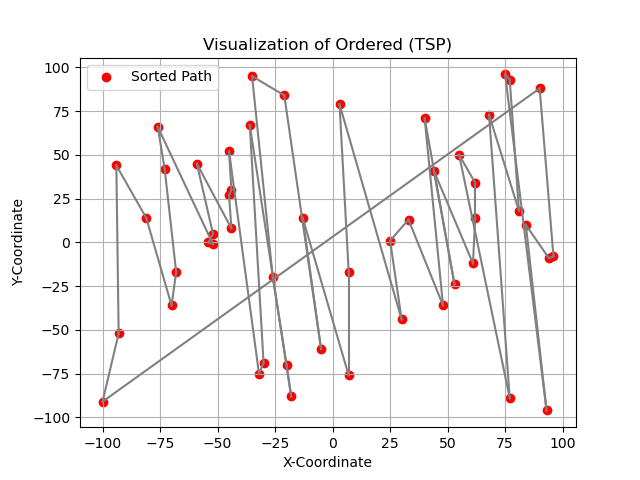
\includegraphics[width=1.1\linewidth]{assets/Img/OrdVisual.png}
            \caption{Ordenación}
            \label{fig:ordered}
      \end{minipage}
\end{figure}
\begin{figure}[H]
      \centering
      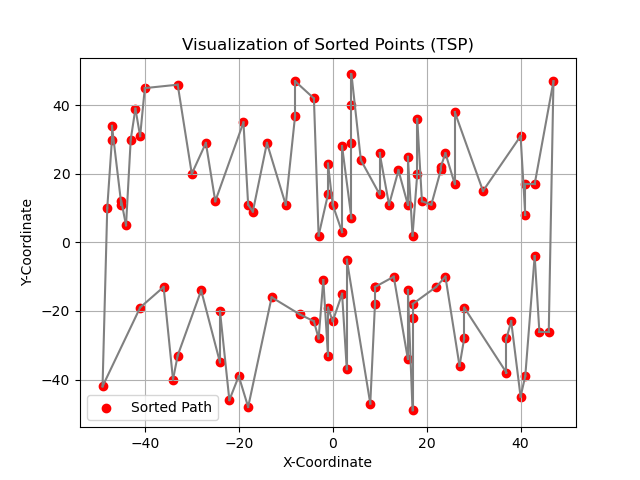
\includegraphics[width=0.6\linewidth]{assets/Img/CircVisual.png}
      \caption{Circular}
      \label{fig:circular}
\end{figure}
Una vez graficadas, podemos ver los problemas principales de cada uno de los algoritmos,
en el caso de \textit{Nearest Neighbour}, se puede apreciar que la distancia de cierre
es muy grande, sin embargo, aparenta un camino parecido al óptimo, en el caso de 
\textit{Ordenación}, se puede apreciar que, mientras los puntos x están cerca, los saltos
en y son muy grandes, y además la distancia de cierre es máxima, en el caso de \textit{Circular},
se puede apreciar que los saltos en y son más pequeños y la distancia de cierre es menor.
\\ \\ 
De este análisis visual, podemos deducir que el algoritmo \textit{Nearest Neighbour} es el
que mejor resultado proporciona, le sigue \textit{Circular} y por último \textit{Ordenación}.
Podríamos dejar el estudio aquí, sin embargo, se proponen maneras de mejorar los algoritmos.
\subsection{Mejoras}
Para mejorar y comparar los algoritmos, comenzamos notando que en el caso de 
\textit{Nearest Neighbour}, la elección del punto de partida nos proporciona un camino
distinto, por lo que, para mejorar la precisión del algoritmo, se puede ejecutar
el algoritmo con distintos puntos de partida y quedarnos con el mejor resultado.
En los casos de \textit{Ordenación} y \textit{Circular}, esto no tendría mucho sentido, 
sin embargo podríamos jugar con la ordenación respecto de un eje u otro, o con la
división en dos partes, respectivamente, para mejorar la precisión de los mismos.
\\ \\
Este tipo de mejoras, son sencillas y no suponen un gran aumento en cuanto al tiempo
de ejecución, sin embargo, tampoco suponen una mejora significativa en cuanto a la
precisión. Su mejor virtud es que nos proporcionan una velocidad de ejecución muy
rápida y una precisión aceptable, por lo que, en la práctica, se recomienda su uso,
sin embargo, habrá aplicaciones en las que se necesite una precisión mayor, en cuyo 
caso se recomienda el uso de algoritmos más complejos como $\lambda$-opt o genéticos.
\subsection{Precisión y Tiempos}
En esta sección se proporcionan los tiempos de ejecución de los algoritmos y se comparan
con la precisión de los mismos, para ello, se han ejecutado los algoritmos sobre un entorno
cuya solución óptima se conoce, de esta forma, se puede comparar la solución obtenida
con la solución óptima, el entorno en cuestión es un conjunto de Paises del mundo
que se han dividido en pueblos y ciudades de interés. A continuación mostramos 
los resultados que hemos obtenido:
\\ \\
Comenzamos exponiendo los resultados que arrojan los algoritmos sin mejoras:
% Dos graficas
\begin{figure}[H]
      \centering
      \begin{minipage}{.48\textwidth}
            \centering
            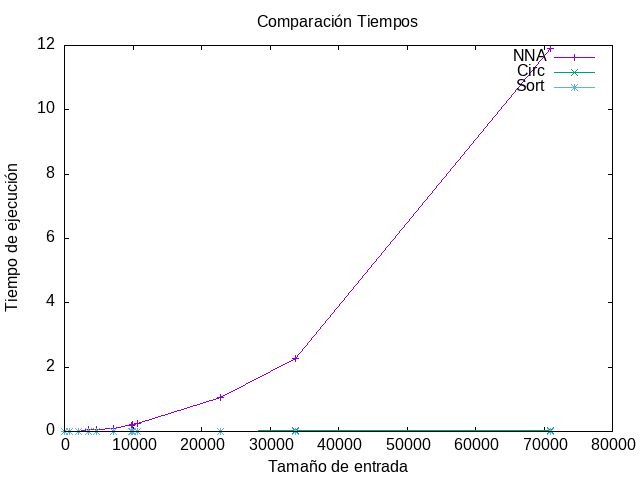
\includegraphics[width=1\linewidth]{assets/Img/Tiempos.png}
            \caption{Tiempos completos}
            \label{fig:nearest}
      \end{minipage}%
      \begin{minipage}{.48\textwidth}
            \centering
            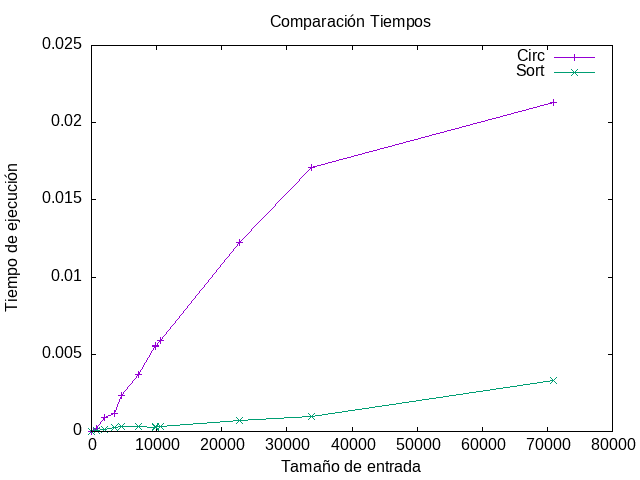
\includegraphics[width=1\linewidth]{assets/Img/TiemposCircSort.png}
            \caption{Tiempos Circ y Sort}
            \label{fig:ordered}
      \end{minipage}
\end{figure}
Como se puede ver, el algoritmo \textit{Nearest Neighbour} es el más lento,
esto era de esperar debido a que, como veremos ahora, es el que mejor precisión
ofrece. El mismo razonamiento se puede aplicar a los algoritmos \textit{Ordenación}
y \textit{Circular}.
Si nos fijamos ahora en los tiempos de ejecución de los algoritmos tras las mejoras,

\begin{figure}[H]
      \centering
      \begin{minipage}{.48\textwidth}
            \centering
            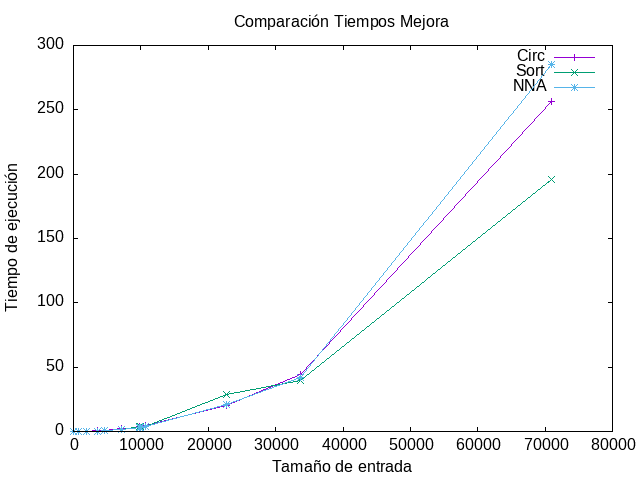
\includegraphics[width=1\linewidth]{assets/Img/TiemposMejora.png}
            \caption{Tiempos completos}
            \label{fig:nearest}
      \end{minipage}%
      \begin{minipage}{.48\textwidth}
            \centering
            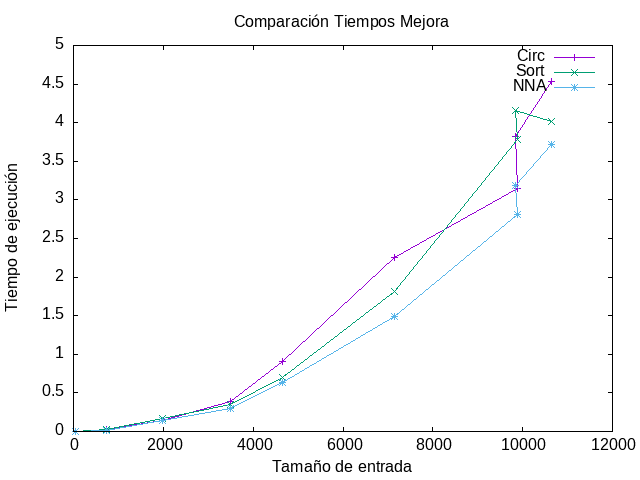
\includegraphics[width=1\linewidth]{assets/Img/TiemposMejoraChico.png}
            \caption{Tiempos menor Tamaño}
            \label{fig:ordered}
      \end{minipage}
\end{figure}
Podemos ver como hay un gran aumento en el tiempo, sin embargo, son tiempos
similares entre ellos, por lo que nos interesa quedarnos con el que mejor precisión
ofrece:
\begin{figure}[H]
      \centering
      \begin{minipage}{.48\textwidth}
            \centering
            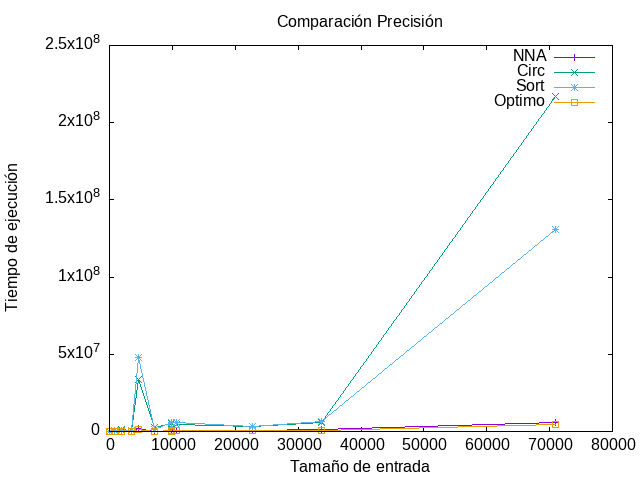
\includegraphics[width=1\linewidth]{assets/Img/Precision.png}
            \caption{Precisión sin mejoras}
            \label{fig:nearest}
      \end{minipage}%
      \begin{minipage}{.48\textwidth}
            \centering
            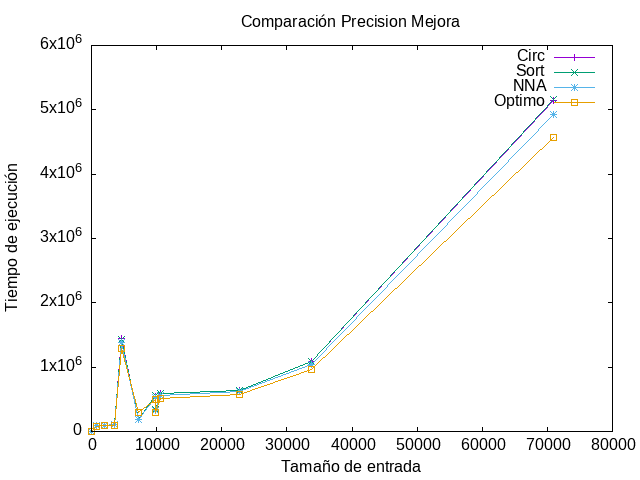
\includegraphics[width=1\linewidth]{assets/Img/PrecisionMejora.png}
            \caption{Precisión tras mejora}
            \label{fig:ordered}
      \end{minipage}
\end{figure}
Como se puede ver, todos los algoritmos con mejora, se quedan muy cerca
de la solución óptima, sin embargo, el algoritmo \textit{Nearest Neighbour}
es el que mejor precisión ofrece, tanto en el caso de mejora como 
en el caso sin mejora, por lo que, en la práctica, se recomienda su uso. Para 
aplicaciones donde la precisión sea un factor crítico, se recomienda el uso
combinado de distintas mejoras como la elección de distintos puntos de partida
o el uso de algoritmos más complejos como $\lambda$-opt o genéticos.

\end{document}